\frame{
  \vspace{-1em}
  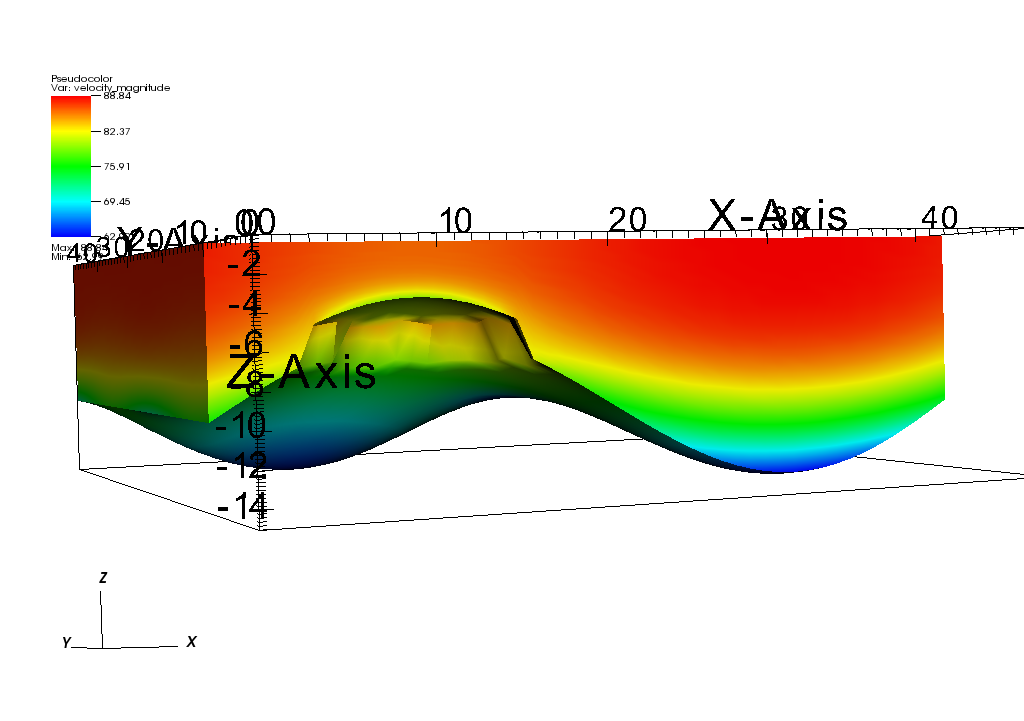
\includegraphics[width=\textwidth]{figures/THI/y-5km-m6p5l4-clip}
  \vspace{-3.5em}
  \begin{itemize}
  \item Bathymetry is essentially discontinuous on any grid
  \item Shallow ice approximation produces oscillatory solutions
  \item Nonlinear and linear solvers have major problems or fail
  \item Grid sequenced Newton-Krylov multigrid works \\
    as well as in the smooth case
  \end{itemize}
}
